\section{Theoretische Grundlagen}
  
  Die Gaschromatographie (GC) ist ein häufig verwendetes Trennverfahren. Im Gegensatz zur Flüssig- keitschromatographie wird als mobile Phase ein inertes Gas verwendet. Die mobile Phase durchströmt ein Rohr, das die stationäre Phase enthält. Aufgrund von unterschiedlich starken Wechselwirkungen der in der mobilen Phase \textit{gelösten} Substanzen mit der stationären Phase kommt es zur Trennung. Die GC eignet sich besonders für leicht flüchtige Verbindungen. \citep[S. 164, 165]{Taschenatlas}
  
  \subsection{Aufbau eines Gas-Chromatographen und Ablauf einer Analyse}
    
    Ein Gaschromatograph besteht aus einer Trägergasversorgung inkl. Strömungsregler,  einer Vorrichtung zur Probenaufgabe, einer Trennsäule, einem Säulenofen, einem Detektor und einem Auswertegerät. Um eine Probe zu analysieren, wird sie über das Injektionsventil in die Trennsäule injiziiert. Das Trägergas agiert als mobile Phase und transportiert die Probe durch die Trennsäule, die die stationäre Phase enthält. Da die Stärke der Wechselwirkungen zwischen Analyt und stationärer Phase temperaturabhängig sind, regelt der Säulenofen die Temperatur gemäß einem festgelegten Temperaturprogramm. Am Ende der Säule passieren die Substanzen zu unterschiedlichen Zeiten einen Detektor. \citep[S. 164, 165]{Taschenatlas}
    
    \subsubsection{Injektionssystem}
      
      Das Injektionssystem hat die Aufgabe, die in einem leicht flüchtigen Lösungsmittel gelöste Probe in die Trennsäule zu überführen. Man unterscheidet zwischen zwei Arten. Beim "on-column injector" geht die Probe von der Injektionsspritze direkt in die Trennsäule/Kapillare über. Beim "split-injector" erfolgt die Probenaufgabe mit einer Injektionsspritze durch ein Septum, das einen luftdichten Übergang von Spritze in das Verdampfungsrohr ermöglicht. Die dort verdampfte Probe wird mithilfe des eingespritzten Trägergases in die Säule transportiert. Der Verdampfungsraum wird unabhängig vom Säulenofen geheizt, um höhere Temperaturen und damit eine unverzögerte Überführung in die Gasphase zu ermöglichen. Die in die Trennsäule strömende Probenmenge kann mit einem Splitter reguliert werden, was vor allem bei Kapillarsäulen wichtig ist. \citep{Versuchsvorschrift}, \citep[S. 164]{Taschenatlas}          
      
    \subsubsection{Mobile Phase - Trägergas}
      
      Die mobile Phase ist ein chemisch inertes Gas. Zum Einsatz kommen in erster Linie Wasserstoff, Stickstoff und Helium. Weitere Anforderungen an das Trägergas sind hohe Reinheit und damit verbunden ein geringer Gehalt an Wasser und Sauerstoff, da diese die Trennsäule beschädigen könnten. \citep{Versuchsvorschrift}, \citep{Taschenatlas}
      
    \subsubsection{Stationäre Phase - Trennsäule}
      
      Als stationäre Phasen eignen sich adsorbierende Festkörper und absorbierende Flüssigkeiten auf einem inertem Trägermaterial. Sie befinden sich in Rohren aus Glas oder Quarz. Man unterscheidet zwischen gepackten Säulen und Kapillarsäulen. Bei der gepackten Säule befindet sich die stationäre Phase auf Trägerpartikeln, die die komplette Säule ausfüllen. Kapillarsäulen sind dünner, länger und nur am Rand mit dem Trägermaterial besetzt. Sie enthalten demnach einen offenen Längskanal. Im Experiment wird eine Kapillarsäule verwendet, weswegen diese im Folgenden näher beschrieben wird. Außerdem erzielen sie sehr hohe Auflösungen und werden deswegen häufig verwendet.
      
      Bei den Kapillarsäulen unterscheidet man zwischen Dünnschichtkapillarsäulen (porous open tubular columns - PLOT), Träger-beschichteten Kapillaren (support coated open tubular columns - SCOT) und Dünnfilmkapillarsäulen (wall coated open tubular columns - WCOT). Dünnschichtkapillarsäulen enthalten eine dünne Schicht des Trägermaterials auf der inneren Seite der Trennsäule, wobei das Trägermaterial mit der flüssigen Phase belegt ist. Sie werden hauptsächlich bei Adsorptions-GC Trennungen verwendet. Bei Dünnfilmkapillarsäulen ist die stationäre Phase (dünner Flüssigkeitsfilm) direkt auf die (aufgeraute) Innenseite der Säule aufgetragen. \citep[S. 164-166]{Taschenatlas} \\
      
      Die Qualität der Trennung hängt stark von den chemischen Eigenschaften der stationären Phase ab, da sie das Retentionsverhalten des Analyten bestimmen. Dabei ist ein wichtiger Faktor die Polarität. Un-/Polare stationäre Phasen wechselwirken mit un/-polaren Substanzen und halten diese somit länger zurück. Die Wahl der stationären Phase richtet sich somit an die Zusammensetzung der Probe und muss gegebenenfalls adaptiert werden. \citep{Versuchsvorschrift}
      
    \subsubsection{Säulenofen}
      
      Der Säulenofen hat die Aufgabe, die Temperatur während der Trennung zu regulieren. Dies ist notwendig, da der Dampfdruck und damit der Verteilungskoeffizient $K$ mit der Temperatur zusammenhängt. Bei Temperaturerhöhung steigt der Dampfdruck logarithmisch an, während sich die Retentionszeit logarithmisch verkürzt. Grundsätzlich sind zwei Temperaturprogramme denkbar. Die isotherme Trennung eignet sich zum Beispiel für homologe Reihen von $n$-Alkanen. Bei der Gradientenmethode wird die Temperatur stufenweise erhöht, was bei Gemischen unterschiedlicher Polarität und Flüchtigkeit von Vorteil ist. \citep[S. 168]{Taschenatlas}   
    
    \subsubsection{Detektor}
    
      Der Detektor befindet sich am Ende der Trennsäule und misst je nach Methode diverse physikalischen Eigenschaften der vorbeiströmenden Substanzen, um diese zu quantifizieren. Im Folgenden werden die wichtigsten Detektoren näher beschrieben. Auf den für phosphor- und stickstoffhaltige Verbindungen ausgelegten Thermionischen Detektor (TID), der eine abgewandelte Form des Flammenionisations-Detektor ist, wird nicht näher eingegangen.
      
        \begin{itemize}
          \item Wärmeleitfähigkeitsdetektor
      
      Der Wärmeleitfähigkeitsdetektor besteht aus zwei Messzellen mit Heizdrähten aus Platin oder Wolfram. Eine Zelle wird von reinem Trägergas und die andere vom aus der Trennsäule kommenden Eluentenstrom durchflossen. Befindet sich ein Analyt im Trägergas, so verringert sich die Wärmeleitfähigkeit des Gasstroms und die Drähte heizen sich auf, was eine Erhöhung des Widerstandes und damit einen messbaren Spannungsabfall bewirkt. Der Detektor ist sehr universell einsetzbar und zerstört die Analyten nicht. \citep[S. 170]{Taschenatlas}
      
          \item Flammenionisations-Detektor (FID)
      
      
      Der Eluentenstrom wird mit Wasserstoff und Luft gemischt und strömt in eine Brennerdüse, wo mit einer Zündspule gezündet wird. Bei der Verbrennung eines Analyten entstehen aus C-C und C-H Bindungen Ionen wie \ch{CHO\pch} (Radikalmechanismus). Aufgrund der Ionen fließt bei angelegter Gleichspannung ein der Analytkonzentration proportionaler Strom zwischen Anode und Kathode, die um die Flamme angeordnet sind. Der FID spricht auf organische Verbindungen mit einer großen Anzahl an C-C und C-H Bindungen an. Verbindungen mit vielen Heteroatomen sowie anorganische Verbindungen lassen sich schlecht bis gar nicht nachweisen. Ein weiterer Nachteil ist, dass die Analytmoleküle zersört werden.\citep{Versuchsvorschrift}, \citep[S. 172]{Taschenatlas}
     
                 
          \item Elektroneneinfang-Detektor (ECD)
          
      Der $\beta$-Strahler \isotope*{63,Ni} emittiert energiereiche Elektronen, die das Trägergas (meist \ch{N2} oder \ch{Ar} mit \SI[mode=text]{5}{\percent} \ch{CH4}) ionisieren. Die freigesetzten Primärelektronen werden durch die angelegte Spannung zwischen Anode und Kathode zur Anode beschleunigt und bewirken einen Nullstrom. Befindet sich ein Analyt mit hoher Elektronenaffinität im Trägergas, fängt er die Elektronen ein und verringert den Stromfluss. \citep{Versuchsvorschrift}
      
          \item Massenspektrometer
      
      Im Massenspektrometer werden die Analyten ionisiert und die Masse durch Beobachtung ihres Verhaltens im elektrischen und magnetischen Feld bestimmt. Über das Fragmentationsmuster können Informationen über die Struktur gewonnen werden, was ein bedeutender Vorteil gegenüber den anderen Methoden ist. \citep{Versuchsvorschrift}
      
        \end{itemize}

  \subsection{Chromatographische Parameter}
    
    Um den Trennvorgang sowie die Trennleistung einer Analyse bzw. einer Säule zu charakterisieren, hat sich eine Vielzahl an Kenngrößen und Parametern etabliert, die im Folgenden beschrieben werden.
    
     Um die Position und das Aussehen eines Peaks zu beschreiben eignet sich die Totzeit $t_0$ (Zeit der Probe in der mobilen Phase), die Bruttoretentionszeit $t_B$ (Zeit der Probe in mobiler und stationärer Phase), die Nettoretentionszeit $t_R$ (Zeit der Probe in der stationären Phase - $t_R = t_B - t_0$), die Basispeakbreit $w$ (Anlegen zweier Tangenten in \SI[mode=text]{60}{\percent} Peakhöhe und Bestimmung des Abstandes der Schnittpunkte mit der Basislinie) und die Peaksymmetrie. 
    
    Wechselwirkungsvorgänge werden durch den Kapazitätsfaktor $k$ (relative Verweildauer des Analyten in stationärer Phase - $k = t_R / t_0$), den Verteilungskoeffizient $K$ ($K = c_S / c_M$ in Analogie zum Massenwirkungsgesetz) und die lineare Strömungsgeschwindigkeit $v$ ($v = L / t_R$ mit Säulenlänge $L$) beschrieben. 
    
    Die Effizienz einer Trennsäule wird durch die theoretische Trennstufenhöhe (Bodenhöhe) $H$ und die Anzahl an theoretischen Böden (Trennstufenzahl) $N$ charakterisiert ($L = N H$). Die Anzahl an theoretischen Böden ist ein Maß für die Anzahl an theoretischen Gleichgewichtseinstellungen des Analyten zwischen mobiler und stationärer Phase und kann u. a. mit 
    
      \begin{equation}
        N = 16 \left(\frac{t_R}{w}\right)^2
      \end{equation} 
    unabhängig von $H$ und $L$ berechnet werden. Die Bodenhöhe in Abhängigkeit von der linearen Strömungsgeschwindigkeit $v$ wird durch die Van-Deemter Gleichung 
    
      \begin{equation}
        H(v) = A + \frac{B}{v} + C v
      \end{equation}
    beschrieben (Beiträge der Eddy-Diffusion $A$, Longitudinaldiffusion $B$ und des verzögerten Massentransfers $C$). \textit{Bild einfügen} Die maximale Trennleistung erfolgt am Minimum der Kurve. 
    
    Die Trennleistung, also die Fähigkeit zwei benachbarte Peaks eindeutig aufzutrennen, wird durch die Auflösung $R = 2\left(t_{R2} - t_{R1}\right) / \left(w_2 + w_1\right)$ und die relative Retention bzw. Selektivität $\alpha = t_{R2} / t_{R1}$ charakterisiert. Desto größer $R$ und $\alpha$ sind, desto  besser ist die Trennung. \citep{Versuchsvorschrift}
    
  \subsection{Kalibrierung über einen internen Standard}
  
    Man benötigt einen Standard, der ähnliche physikalische und chemische Eigenschaften wie die Probe besitzt. Zur Kalibrierung werden mehrere Lösungen mit jeweils gleicher Standardkonzentration $c_{S}$, jedoch unterschiedlichen Probenkonzentrationen $c_{P}$ hergestellt und die Signalhöhen von Standard $S_{S}$ und Probe $S_{P}$ gemessen. In einem Diagramm wird auf der Ordinate die Signalhöhe und auf der Abszisse das Verhältnis von Proben- zu Standardkonzentration aufgetragen. Durch umstellen der Kalibriergeraden 
    
      \begin{equation}
        \frac{S_{P}}{S_{S}} = b \frac{c_{P}}{c_{S}} + a
      \end{equation}
    kann bei der tatsächlichen Messung die Probenkonzentration bei bekannter $c_S$ berechnet werden (Fitparameter $a$ und $b$). Der Response-Faktor wird durch
    
      \begin{equation}
        R_f = \frac{c_{P}}{c_{S}} / \frac{S_{P}}{S_{S}}
      \end{equation}
    definiert. Die Methode des internen Standards ist sehr robust, da systematische Fehler meist sowohl Probe als auch Standard betreffen und damit das Signalverhältnis gleich bleibt. \citep{AnalytikIII} 
    
  %\begin{figure}[H]
    %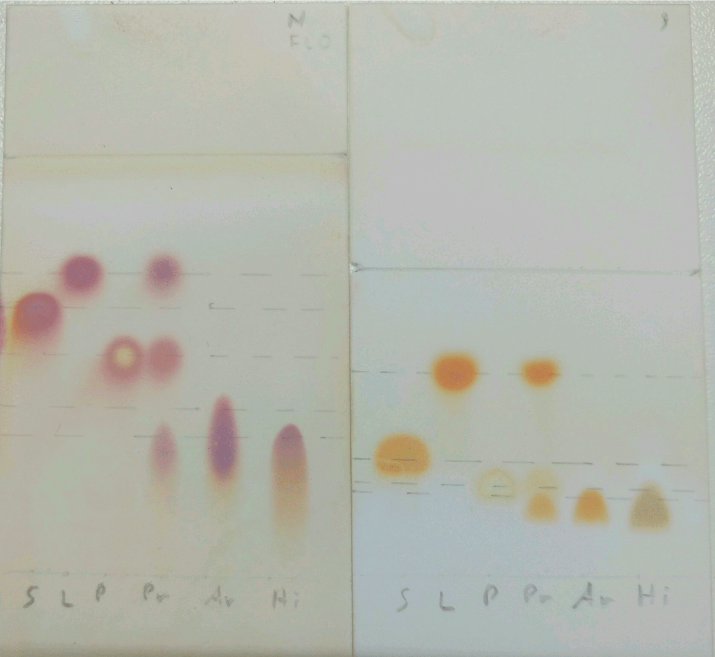
\includegraphics[scale=0.25, center]{images/test.png} 
    %\caption[Quelle: Autor]{Test}
    %\label{fig:Test}
  %\end{figure}
      